\begin{problem}
  \begin{enumerate}
    \item What is the best approximation to $f(x) = x$ from
      $\mathcal{P}_3$?
    \item What is the best approximation to $f(x) = \|x\|$ on $[-1, 1]$
      from $\mathcal{P}_1$?
  \end{enumerate}
\end{problem}

\begin{solution}
  \begin{enumerate}
    \item As $x \in \mathcal{P}_3$ the best approximation to $x$ is
      $x$.
    \item Firstly we assume that the norm to be used is the
      $\infty$-norm. The best approximation can then be found by
      inspection to be $g(x) = \frac{1}{2}$ with $\|(\frac{1}{2} -
      \|x\|)\|_\infty = \frac{1}{2}$. There are only two free
      parameters in the elements of $\mathcal{P}_1 = \{y(x)= \alpha +
      \beta x:\alpha,\beta \in \mathds{R}\}$. Note that the maximum of
      a straight line (and thus differences of such) must be on the
      limits of the interval. In this case it means that we may only
      consider the points $x=-1, 0, 1$ when discussing the
      $\infty$-norm in this case.
      
      We have that $\alpha > \frac{1}{2} \Rightarrow \|(y(x) -
      \|x\|)\|_\infty > \frac{1}{2}$ as the difference at $x=0$ is
      solely determined by $\alpha$. Also, if $\alpha < \frac{1}{2}$
      the difference at one of the endpoints of the interval will be
      larger than $\frac{1}{2}$. Thus the best approximation have
      $\alpha=\frac{1}{2}$.

      \begin{figure}[!ht]
        \centering \includegraphics[scale = 0.1]{drawing_task_6.png}
        \label{fig:task_6}
      \end{figure}

      Finally, to conclude the argument, $\beta \neq 0$ will result in
      the difference at either $x=-1$ or $x=1$ becoming the new
      maximum. Thus $\beta = 0$
  \end{enumerate}
\end{solution}

 
%%% Local Variables:
%%% TeX-master: "report.tex"
%%% End:
